\documentclass{amsart}
\usepackage{amssymb, amsmath, graphicx, caption, enumerate}
\graphicspath{ {images/} }
\usepackage{amsthm}
\usepackage{xargs}
\usepackage{scalerel}



\newcommand{\D}{\mathcal{D}}
\newcommand{\A}{\mathcal{A}}
\newcommand{\N}{\mathbb{N}}
\newcommand{\Z}{\mathbb{Z}}
\newcommand{\R}{\mathbb{R}}
\newcommand{\K}{\mathbb{K}}
\newcommand{\C}{\mathbb{C}}
\newcommand{\ds}{\displaystyle}
\newcommand{\op}[1]{\left(#1\right)}
\newcommand{\cp}[1]{\left[#1\right]}
\newcommand{\av}[1]{\left| #1\right|}
\newcommand{\st}[1]{\left\{#1\right\}}


\usepackage[colorinlistoftodos,prependcaption,textsize=tiny]{todonotes}
\newcommandx{\question}[2][1=]{\todo[linecolor=red,backgroundcolor=red!25,bordercolor=red,#1]{#2}}
\newcommandx{\change}[2][1=]{\todo[linecolor=blue,backgroundcolor=blue!25,bordercolor=blue,#1]{#2}}
\newcommandx{\add}[2][1=]{\todo[linecolor=OliveGreen,backgroundcolor=OliveGreen!25,bordercolor=OliveGreen,#1]{#2}}
\newcommandx{\improve}[2][1=]{\todo[linecolor=Plum,backgroundcolor=Plum!25,bordercolor=Plum,#1]{#2}}
\newcommandx{\thiswillnotshow}[2][1=]{\todo[disable,#1]{#2}}
\newcommandx{\remove}[2][1=]{\todo[linecolor=yelllow,backgroundcolor=yellow!10,bordercolor=red,#1]{#2}}


\newcommand\reallywidehat[1]{\arraycolsep=0pt\relax%
\begin{array}{c}
\stretchto{
  \scaleto{
    \scalerel*[\widthof{\ensuremath{#1}}]{\kern-.5pt\bigwedge\kern-.5pt}
    {\rule[-\textheight/2]{1ex}{\textheight}} %WIDTH-LIMITED BIG WEDGE
  }{\textheight} % 
}{0.5ex}\\           % THIS SQUEEZES THE WEDGE TO 0.5ex HEIGHT
#1\\                 % THIS STACKS THE WEDGE ATOP THE ARGUMENT
\rule{-1ex}{0ex}
\end{array}
}

\setlength{\textwidth}{\paperwidth}
\addtolength{\textwidth}{-2.75in}
\calclayout

\setcounter{secnumdepth}{0}
\usepackage{titlesec}
\titleformat{\section}{\center\large\bfseries}
\titleformat{\subsection}{\center}


% TOC
\setcounter{tocdepth}{1}


\begin{document}





\begin{abstract}

Obtaining the solution to stochastic inverse problems is an important challenge in computational science. By solving a stochastic inverse problem, one may find an updated  characterization of parameter space that combines  prior beliefs and observable data. Using a new approach detailed in \cite{BJW18a}, we may solve for a probability distribution in parameter space, $\Lambda$, such that its push-forward %(i.e. image) 
through the parameter-to-data map $f(\lambda)$ matches the observed probability density on the data space, $\mathcal{D}$. 
Under certain conditions \cite{BJW18a, Tarantola}, 
an approximate solution of the stochastic inverse problem can be obtained as the solution of a regularized, convex minimization problem.
  
In this proposal, we consider a noisy map $f$ from a high-dimensional $\Lambda$ to $\mathcal{D}$ of specified dimension, where the gradient of $f$ exists, but may be inaccessible. If the gradient of $f$ is accessible, the minimization problem can be solved using gradient-based descent methods. If the gradient of $f$ is inaccessible, one may apply Derivative-Free Optimization (DFO) schemes as in \cite{CW}. In either case,  the effectiveness of the optimization algorithm may be enhanced by performing dimension reduction in $\Lambda$ as in \cite{Constantine2015, Russi}. 
We consider different strategies for computing the active subspace of $f$ in the context of both approaches, and apply them to the data-consistent inversion of two model problems. Both of these model problems are related to stochastic inverse problems 
arising in the simulation of plasmas in fusion reactors.
 

\end{abstract}


\title{Thesis Proposal}

\author{Jordan R. Hall}

\maketitle



\tableofcontents

\setcounter{tocdepth}{0}




\newpage

\section{Literature Review and Framework}

In this section we provide a literature review of inverse problem theory, derivative-free (DF) optimization, and dimension reduction. 
In the process, we will build a theoretical framework upon which we will pose research questions, state initial results, and form a research plan. 

We begin our discussion by defining a parameter space $\Lambda$ of dimension $N$, a map or ``model" $f$, and a data space $\mathcal{D}$. We assume that $\mathcal{D}$ has dimension $M$, typically with $M\leq N$. Points in $\mathcal{D}$ may be known values of $f(\lambda), \lambda\in \Lambda$; as such, we may write $d=f(\lambda)$ to denote the particular datum corresponding to the evaluation of a point $\lambda \in \Lambda$ under $f$. Points in $\mathcal{D}$ may also be \textit{observed} data, denoted $d_{\text{obs}}$, where the corresponding $\lambda\in \Lambda$ may be unknown. We allow for realizations of $f$ to be  noisy. Hence, we may model draws of $f$ with $\hat{f}(\lambda)=f(\lambda)+\epsilon$, which is an additive noise structure, or $\hat{f}(\lambda)=f(\lambda)(1+\epsilon)$, which is a multiplicative noise structure.


\subsection{Data-Consistent Inversion}


We follow \cite{BJW18a, Stuart, Tarantola} to formulate an inverse problem in the described setting. Then, we briefly present the data-consistent solution; we refer to \cite{BJW18a} for details.

First, we assume we have prior knowledge of the parameter space, given by the \emph{prior distribution}, $\pi_\Lambda^\text{prior}(\lambda)$. In practical applications, a prior distribution may be given by application experts, but may also reflect the state of knowledge on $\Lambda$ obtained by other mathematical or statistical processes. Second, we assume that we have an \emph{observed density}, $\pi_\mathcal{D}(d)$, which represents our uncertain state of knowledge of observed data and is uncertain due to noise in $f$ and potential measurement error. Informally, the inverse problem is the task of finding an \emph{updated} probability distribution, $\pi_\Lambda^\text{update}$, in $\Lambda$ space that combines the given prior information and data.

It has been shown \cite{BJW18a} that the \textit{classical Bayesian} or \textit{statistical Bayesian} solution to the inverse problem is not generally a 
\textit{pull-back probability measure}, meaning the image of the updated distribution $\pi_\Lambda^\text{update}$ under the map $f$, called the push-forward, is not equal to (and often not ``close" to) the observed probability distribution, $\pi_\mathcal{D}$. 



Given a distribution on $\lambda \in \Lambda$, the \emph{forward Uncertainty Quantification (UQ) problem} is finding the probability distribution of $f(\lambda)$. The forward UQ problem is, in its own right, a nontrivial and important problem in uncertainty quantification. As it turns out, performing DCI will require solving a forward UQ problem. 

Data-consistent inversion (DCI) seeks an updated solution $\pi_\Lambda^\text{update}$ for which the push-forward exactly equals $\pi_\mathcal{D}$. To obtain such a solution, it is necessary to compute the push-forward of $\pi_\Lambda^\text{prior}$. We may form the push-forward of the prior by solving the corresponding forward problem; with certain assumptions on $f, \Lambda,$ and $\mathcal{D}$ the forward problem may be straightforward, with other assumptions, this problem is non-trivial. We denote the solution to the forward problem with $\pi_\mathcal{D}^{f(\Lambda)}$. Then, the \textit{data-consistent} solution to the inverse problem is

\begin{equation} \label{eq:1}
\pi_\Lambda^\text{update}(\lambda)=\pi_\Lambda^\text{prior}(\lambda)\frac{\pi_\mathcal{D}(f(\lambda))}{\pi_\mathcal{D}^{f(\Lambda)}(f(\lambda))}.
\end{equation}

\subsection{Optimization Methods for Solving Inverse Problems}

With our assumptions of an expensive $f$ and a high-dimensional parameter space $\Lambda$, approximately solving the forward problem to obtain the push-forward density generally requires some type of  density estimation, which converges slowly, at best  near Monte Carlo rates of $ \frac{1}{\sqrt{N}}$. As in \cite{Tarantola}, depending on $f$, the solution to the inverse problem can be obtained exactly or approximately by solving an equivalent deterministic convex optimization problem. We may alter the  classical formulation of the deterministic optimization problem to ensure we obtain, depending on $f$, the \textit{data-consistent} (exact or approximate) solution to the inverse problem.

We begin by examining the classical 
formulation of a deterministic optimization problem which corresponds to, for linear models with Gaussian priors and data,  
solving the stochastic inverse problem (SIP) under consideration. In particular, for a linear map $f$, the exact solution is obtained; for nonlinear maps, we obtain an approximate solution. As in \cite{Tarantola}, given observed data $d_{\text{obs}} \sim \pi_\mathcal{D}$ and a draw $\lambda_\text{prior}\sim \pi_\Lambda^\text{prior}$, we define a \textit{misfit function}

\begin{equation} \label{eq:2}
S(\lambda)=\frac{1}{2}\left(||f(\lambda)-d_{\text{obs}}||_\mathcal{D}^2+||\lambda-\lambda_{\text{prior}}||_\Lambda^2\right).
\end{equation}



The misfit function appears in the classical (i.e., statistical Bayesian) solution to the inverse problem, as $\pi_\Lambda^\text{update}(\lambda) \sim \exp(-S(\lambda)).$ 
%We observe
%that finding the MAP point is equivalent to finding the $\lambda$ for which $S$ is minimized.
As in the preceding section, we assume $\pi_\Lambda^\text{prior}$ is a known probability density with mean $\bar{\lambda}$ and covariance matrix $C_\Lambda$; likewise, $\pi_\mathcal{D}$ is a known probability density with mean $\bar{d}$ and covariance matrix $C_\mathcal{D}$. As in \cite{Tarantola}, we can use the assumed covariance structures on $\Lambda$ and $\mathcal{D}$ to rewrite \eqref{eq:2} as


\begin{equation} \label{eq:3}
S(\lambda)=\frac{1}{2}\left(\left|\left|C_\mathcal{D}^{-1/2}(f(\lambda)-d_{\text{obs}})\right|\right|_2^2+\left|\left|C_\Lambda^{-1/2}(\lambda-\lambda_{\text{prior}})\right|\right|_2^2\right).
\end{equation} 

In \cite{Tarantola}, it is assumed that $\pi_\Lambda^\text{prior}$ and $\pi_\mathcal{D}$ are Gaussians, and the misfit function is specified by $\lambda_{\text{prior}}=\bar{\lambda}$ and $d_{\text{obs}}=\bar{d}$ in our notations. In \eqref{eq:2} and \eqref{eq:3}, we choose to define a more general misfit function, so that we may consider the ``misfit" given any draws $\lambda_{\text{prior}}\sim \pi_\Lambda^\text{prior}$ and $d_\text{obs} \sim \pi_\mathcal{D}$. The misfit function defined above can be understood term-by-term. Given $\lambda \in \Lambda$, the term $||f(\lambda)-d_{\text{obs}}||_\mathcal{D}^2$ corresponds to finding the mismatch between the observed $d_\text{obs}$ and $f(\lambda)$ in data space; the term $||\lambda-\lambda_{\text{prior}}||_\Lambda^2$ corresponds to performing Tikhonov regularization, which improves conditioning in minimizing $S$ over $\Lambda$. The minimum of $S$ is typically referred to as the maximum a posteriori point or \textit{MAP point}.

In \cite{wildeyprez},  $S$ is rewritten to obtain a data-consistent MAP point. 
An additional ``deregularization" term is appended so that if a unique solution exists, the regularization will be ``turned off." For now, we assume that $f$ is linear (or can be linearized locally \cite{Smith, Tarantola}), and write the matrix $A$ to define that action of $f$ on $\Lambda$. We also assume that $\pi_\Lambda$ and $\pi_\mathcal{D}$ are Gaussian. In this case, we write the \textit{data-consistent misfit function,}




\begin{equation} \label{eq:4}
T(\lambda)=\frac{1}{2}\left(\left|\left|C_\mathcal{D}^{-1/2}(f(\lambda)-d_{\text{obs}})\right|\right|_2^2+\left|\left|C_\Lambda^{-1/2}(\lambda-\lambda_{\text{prior}})\right|\right|_2^2-\left|\left|C_A^{-1/2}(f(\lambda)-f(\lambda_{\text{prior}}))\right|\right|_2^2\right),
\end{equation} 

\noindent where $C_A=AC_\Lambda A^T$. We note that in the case that $\pi_\Lambda$ and $\pi_\mathcal{D}$ are Gaussian and $f$ is linear, the data-consistent solution to our inverse problem is given exactly by $\pi_\Lambda^\text{update}(\lambda)\sim c \exp(-T(\lambda))$, where $c$ is a constant. Generally, the deregularization term will ensure a solution that updates the distribution on $\Lambda$ only in the directions in which the data is informative. The linear case illustrates the action of the un-regularization term. In the case that a unique solution to the inverse problem exists for a linear $f$ (i.e., $N=M$ and $A$ is full rank), the un-regularization term will equal the Tikhonov regularization term, so that the MAP point solves the data misfit exactly. When the problem is under-determined ($N>M$), then with a linear $f$, the data-consistent solution to inverse problem will lie in a hyperplane in $\Lambda$ containing all the possible points that could have produced the $M$ observed data. Regardless of whether $N=M$ or $N>M$, the MAP point obtained by minimizing the classical misfit, in general, will not be a point that could have produced the observed data. We highlight the difference in solutions in the example below.

\vspace{.125cm} 

\noindent \textbf{Example 1.} \textit{Let $f(\lambda)=2\lambda$, $\lambda_\text{prior}=0.1$, $C_\Lambda=[0.5],$ $d_\text{obs}=0.25$, and $C_\mathcal{D}=[0.25]$; note, $N=M=1$. Then we find that $S(\lambda)=2((2\lambda-0.25)^2+(\lambda-0.1)^2)$, which is minimized by $\lambda^*_S=3/25$. Assuming that $\lambda_\text{prior}$ and $d_\text{obs}$ are the means of Gaussians with variances corresponding to the above covariance matrices, we have $\pi_\Lambda^\text{post} \sim c \exp(-S(\lambda))$ with mean $\lambda_S^*$. Notice $f(\lambda^*_S)=6/25\neq d_\text{obs}$. We write $T(\lambda)=2(2\lambda-0.25)^2$, which is minimized by $\lambda^*_T=1/8$. Notice $f(\lambda^*_T)=d_\text{obs}$. With Gaussian assumptions on the prior and data, we have $\pi_\Lambda^\text{post} \sim c \exp(-T(\lambda))$ with mean $\lambda_T^*$.}



\vspace{.125cm}

In the preceding example, we observe for linear $f$ and $N=M$, the classical MAP point, given by $\lambda_S^*=0.12$ and obtained by minimizing $S$, strikes a balance between the prior belief that $\lambda=0.1$ and the fact that the value $\lambda=0.125$ is the pre-image of $0.25$ under $f$, the observed data point. The data-consistent MAP point, given by $\lambda_T^*=0.125$, is exactly the pre-image of $d_\text{obs}$. Indeed, since the linear map $A$ is full rank in Example 1, the third term in \eqref{eq:3} fully deregularizes (cancels out) the second term, so that the minimum of $T$ is actually just the minimum of the first term, the data mismatch. We see here that classical Bayesian inverse problem theory and DCI pose and answer different questions. For a similar, concrete example where the number of parameters $N$ is greater than the number of data, $M$ (so that the problem is under-determined), we present the following example adapted directly from \cite{BJW18a}.

\begin{figure} 
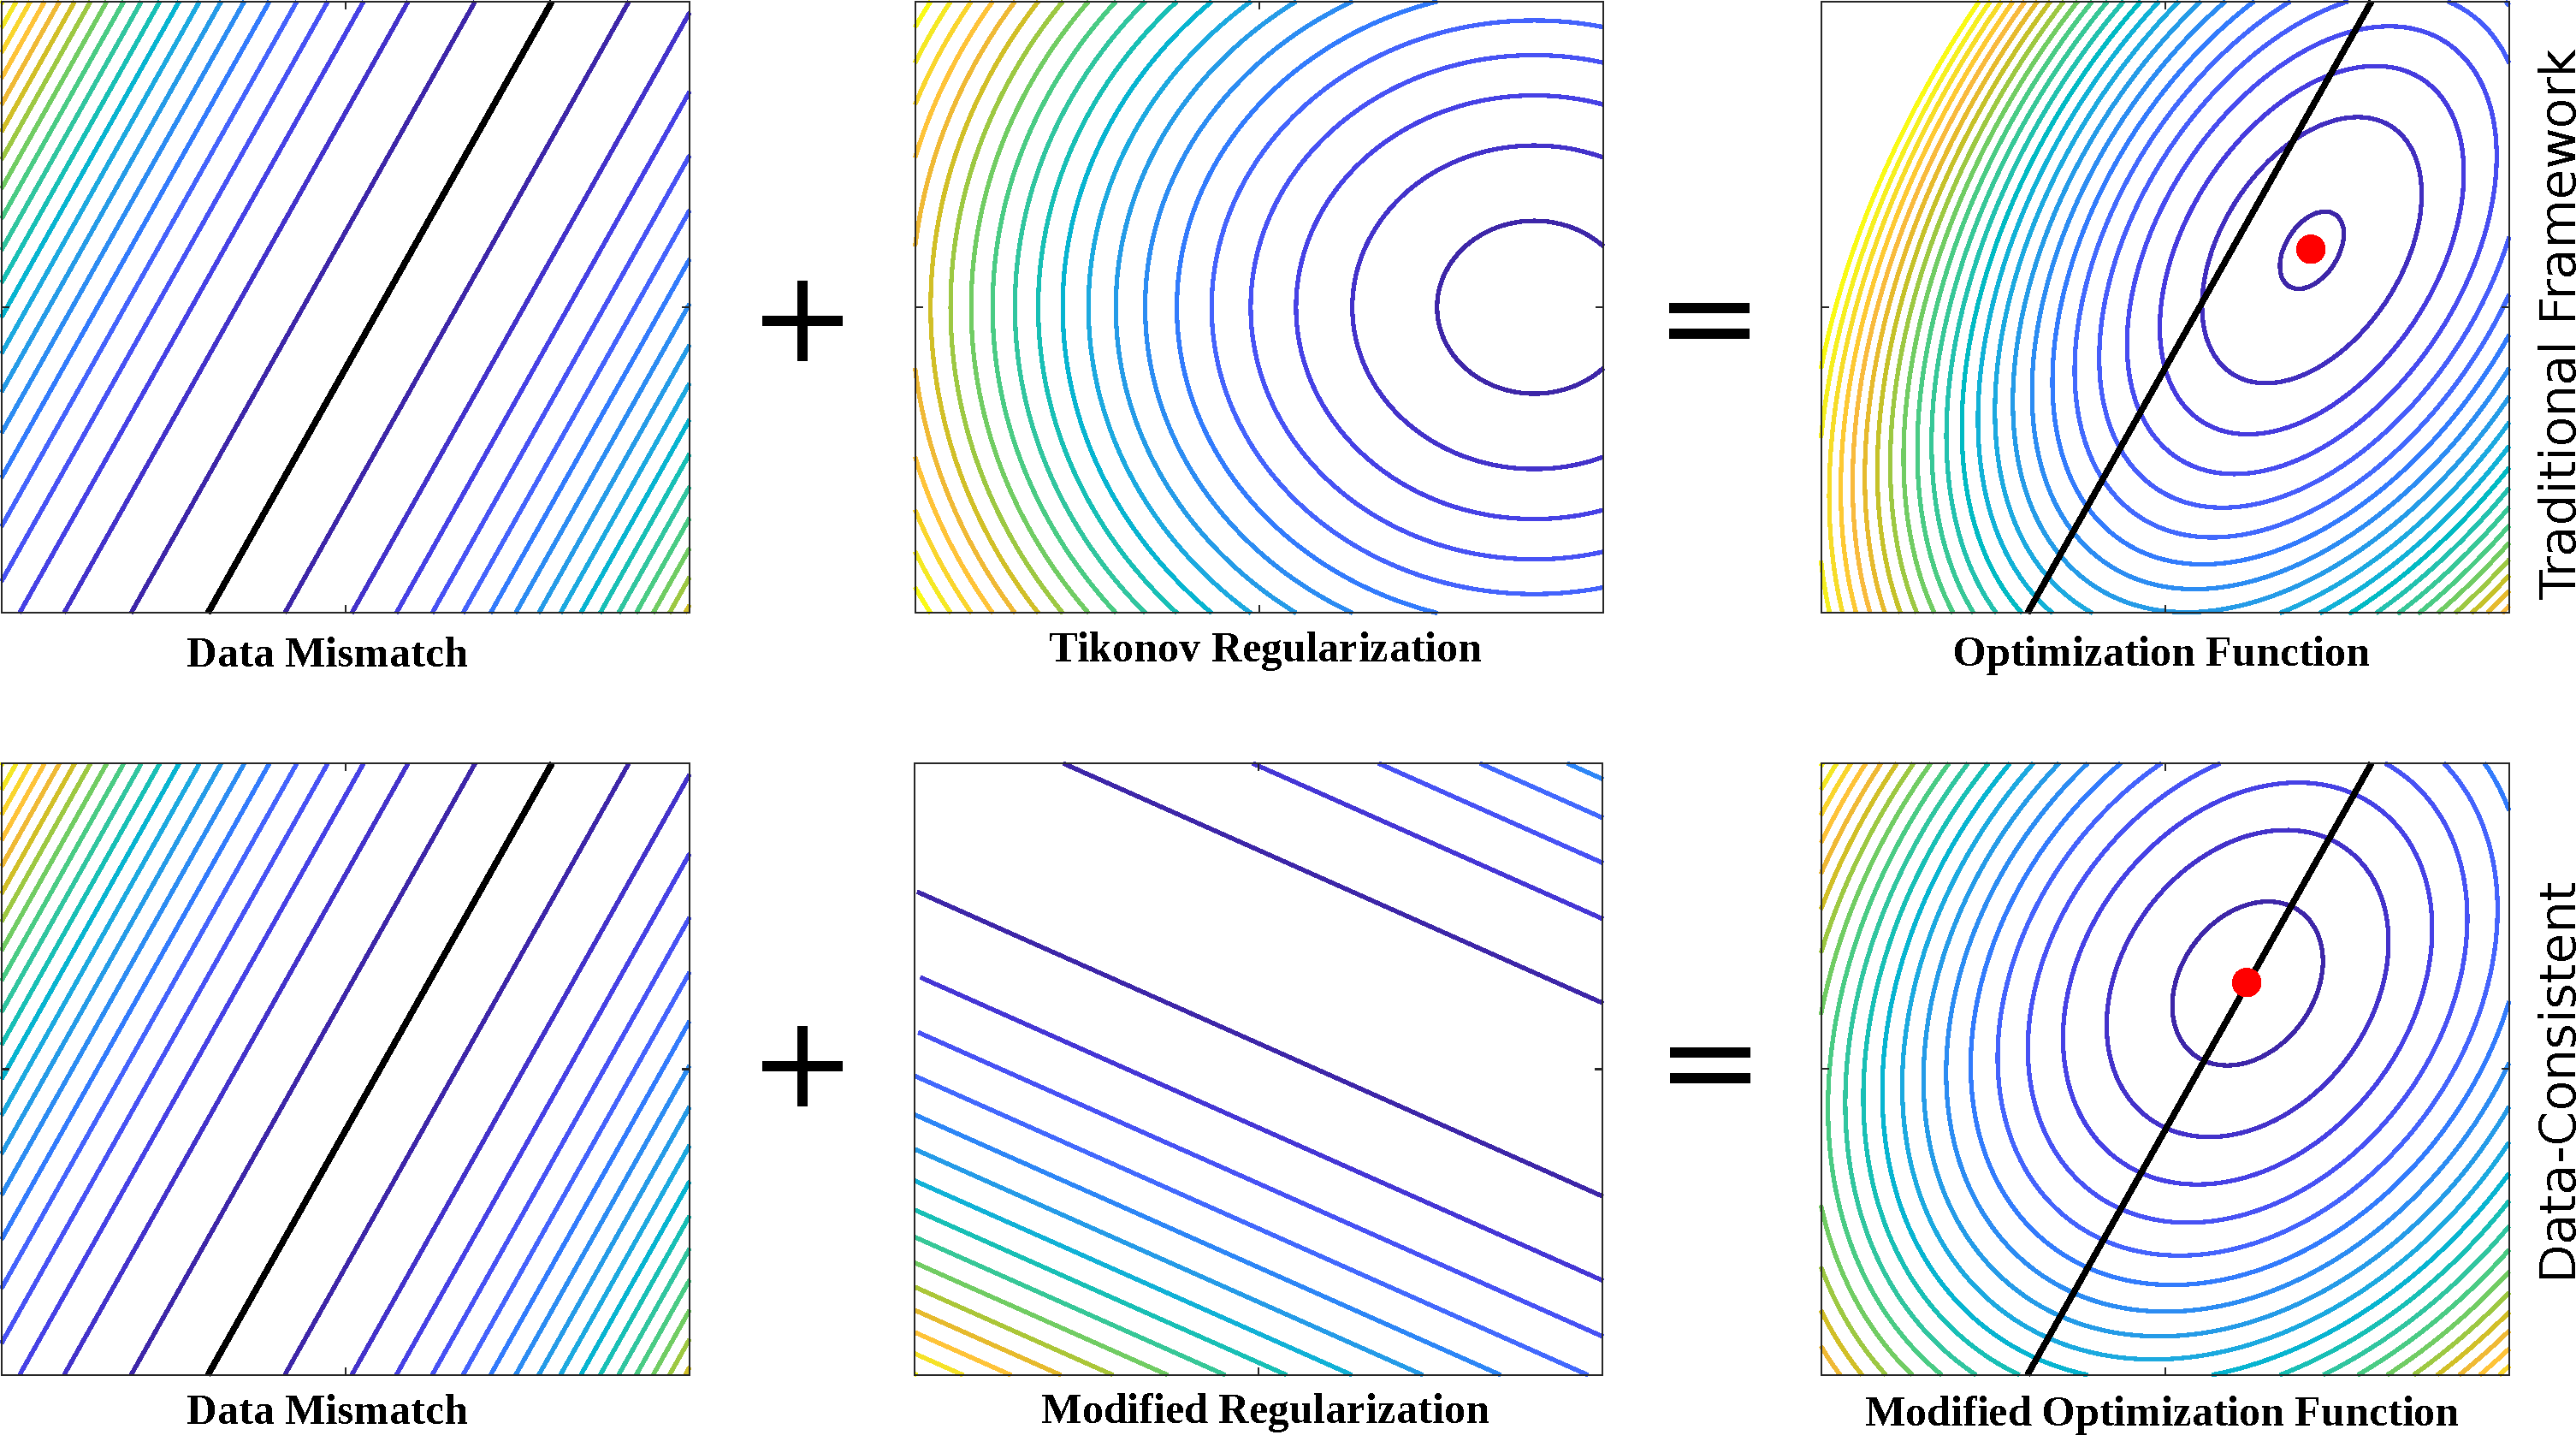
\includegraphics[width=\textwidth]{Regularization-all-in-one.pdf}

\textbf{Figure 1:} This figure from \cite{wildeyprez} shows the process of obtaining the statistical/classical Bayesian solution and data-consistent solution from solving the equivalent deterministic optimization problem corresponding to Example 2.
\end{figure}

\vspace{.125cm} 

\noindent \textbf{Example 2.} \textit{Let $f(\lambda)=2\lambda_1-\lambda_2$, $\lambda_\text{prior}=(0.1 \quad 0.2)^\top$, $C_\Lambda=\text{diag}[0.5,0.25],$ $d_\text{obs}=0.1$, and $C_\mathcal{D}=[0.25]$. Note that with $N>M$, we have an under-determined problem; in this case with $N=2$ and $M=1$, for any $\lambda \in \Lambda$, $f(\lambda)=d=2\lambda_1-\lambda_2$. Since there is just a single $d_\text{obs}$, we have $0.1=2\lambda_1-\lambda_2$.
We find $$S(\lambda)=2(2\lambda_1-\lambda_2-0.1)^2+(\lambda_1-0.1)^2+2(\lambda_2-0.2)^2,$$ 
which is minimized by $\lambda^*_S=(7/50,19/100)$. 
Assuming that $\lambda_\text{prior}$ and $d_\text{obs}$ are the means of Gaussians with variances corresponding to the given covariance matrices, we have $\pi_\Lambda^\text{post} \sim c \exp(-S(\lambda))$ with mean $\lambda_S^*$. 
Notice $f(\lambda^*_S)=9/100\neq d_\text{obs}$. In the data-consistent formulation, we have 
$$T(\lambda)=2(2\lambda_1-\lambda_2-0.1)^2+\frac{1}{9}\left((\lambda_1-0.1)^2+8(\lambda_1-0.1)(\lambda_2-0.2)+16(\lambda_2-0.2)^2\right),$$ 
which is minimized by $\lambda^*_T=(13/90,17/90)$. Notice $f(\lambda^*_T)=d_\text{obs}$. With Gaussian assumptions on the prior and data, we have $\pi_\Lambda^\text{post} \sim c \exp(-T(\lambda))$ with mean $\lambda_T^*$. Figure 1 shows plots of $\lambda_S^*$ and $\lambda_T^*$ along with the relevant visualizations of the terms in $S$ and $T$.} 



\vspace{.125cm}




In the example above, we see that the single datum $d_\text{obs}=0.1$ could be observed by any point $\lambda$ on the line $\lambda_2=2\lambda_1-0.1$, represented by the solid black line seen in several plots in Figure 1. The left-hand plots in Figure 1 are identical, since the data mismatch term in $S$ and $T$ are equal. The Tikhonov regularization term is depicted in the top-middle plot, and the top-right panel shows the corresponding classical Bayesian solution with the MAP point $\lambda_S^*$ shown as a red point and contours corresponding to the updated (Gaussian) prior distribution $c \exp(-S(\lambda))$. 
Just as we saw analytically in Example 2, we see that $\lambda_S^*$ does not lie on the black line representing data-consistent solutions. The action of the modified regularization -- ie, the last two terms in \eqref{eq:4} -- is shown in the bottom-middle plot. Notice that the modified regularization is constant along directions perpendicular to the data, hence, the updated prior will be formed with prior information used only in directions that data is not informative. Thus, it is ensured that $\lambda_T^*$ will lie on the line of data-consistent solutions, as seen in the bottom-right plot in Figure 1, where $\lambda_T^*$ is represented as a red point and the data-consistent solution is given by contours of $c \exp(-T(\lambda))$.


So far, we have presented a deregularization term in \eqref{eq:3} which will hold only for linear (or linearizable) $f$ and Gaussian assumptions on the parameter and data spaces. For general nonlinear functions $f$, the deregularization must be rewritten. Here, we arrived at an open research question, which we discuss further in the proceeding section.



\subsection{Dimension Reduction}
We consider functions from a high-dimensional space $\Lambda$ to a data space of smaller dimension. Many functions of interest %in this paper 
actually represent postprocessed quantities from the solution of complex physical models. %involving quire function evaluations, which are generally expensive due to the many parameters. 
It is not often the case that every parameter has an equal impact on function values; usually some parameters matter more than others. If it is possible to mimic the response of $f$ by processing fewer parameters, we can expect computational savings in many of the problems (i.e., minimization and forward problems) considered here.

In our setting, it may be advantageous to perform dimension reduction on $f$. In particular, we shall consider Active Subspace methods described by Paul Constantine in \cite{Constantine2015} and an equivalent method by T.M. Russi in \cite{Russi}. These techniques seek to explain outputs $f(\Lambda)$ in a subspace $\A \subset \Lambda$ for which the $\dim (\A) <N$. Here we discuss the theoretical formulation of $\A$, but also how it may be found in practice.

We begin by noting $\nabla f(\lambda)\in \Lambda$ is a column vector of the same dimension as inputs $\lambda$ with rows containing the $N$ partial derivatives of $f$, which for this discussion we assume exist, and are square integrable in $\Lambda$ equipped with some probability density that is positive everywhere in $\Lambda$ and 0 otherwise; for instance, we could consider $\pi_\Lambda^\text{prior}(\lambda)$, the density describing our prior state of knowledge, which we choose to abbreviate as $\pi_\Lambda$. %for this discussion. 
In classical active subspace analysis, one transforms inputs $\lambda$ to the origin with some fixed variance, typically so that $\lambda\in [-1,1]^N$. Then, as in \cite{ConstantineMC}, we may write

\begin{equation} \label{eq:5}
W=\int_\Lambda \nabla f(\lambda) \nabla f(\lambda)^\top  \pi_\Lambda(\lambda) d\lambda,
\end{equation} 

\noindent which is an $N\times N$ symmetric positive semi-definite matrix which defines a certain covariance structure of $\nabla f$ over $\Lambda$. This interpretation of \eqref{eq:5} leads one to the idea of computing the Singular Value Decomposition of $W$,

\begin{equation} \label{eq:6}
W=U\Sigma V^*,
\end{equation} 

\noindent where $U$ is $N \times N$ unitary, $\Sigma$ is $N \times N$ diagonal with the singular values of $W$ along its diagonal, and $V^*$ is $N \times N$ unitary. With the singular values of $W$ in hand, we search for a drop-off in the spectrum of $W$. In detail, we plot the singular values, $\{\sigma_i\}_{i=1}^n$ and seek a drop-off in magnitude between some pair of singular values, $\sigma_{j}$ and $\sigma_{j+1}$. The active subspace is the span of $u_1,\ldots,u_{j}$, which are the first $j$ columns of $U$, the left singular vectors of $W$. 

The fact that $u_1,\ldots,u_{j}$ correspond to the nontrivial singular values is exactly why they account for the most amount of variance in function values. In fact, one can view active subspace analysis as an artful choice of principal components after a \textit{full} Principal Component Analysis (PCA) is performed in the gradient space $W$; for more details on this viewpoint, we refer the interested reader to Section 6.4 in \cite{Russi}.

For a point $\lambda \in \Lambda$, we define

\begin{equation} \label{eq:7}
  \mathcal{P}_\A(\lambda)=\sum_{i=1}^{j}\left( u_i^T \lambda\right)u_i \in \A, 
\end{equation}

\noindent which is a projection of the point $\lambda$ in the active directions of $f$. We call this projection an \textit{active variable}, which is a point in the active subspace $\A$. We have arrived at the property that 

\begin{equation} \label{eq:8}
f\left(\mathcal{P}_\A(\lambda)\right) \approx f(\lambda).
\end{equation}

In practice, finding an active subspace of $f$ will require forming an approximation to $W$ in a Monte Carlo fashion; see \cite{ConstantineMC}. We choose to present a Monte Carlo approach that is simple to implement, as in \cite{Russi}. In short, for a random draw $\lambda_i \in \Lambda$, we will find its evaluation under the approximate or analytic gradient (depending on whether we have $\nabla f$ analytically), and store the row vector $\nabla f(\lambda_i)^\top$ in a matrix with an SVD corresponding to \eqref{eq:6}, up to scaling.

In the following, we assume that we lack an analytic form of $\nabla f$; if the analytic gradient is available, the proceeding Monte Carlo method remains valid, and all notations corresponding to approximating $\nabla f$ may be dropped.


One initializes the method by performing $S$ random draws of $\lambda_i \in \Lambda$. We then compute $f(\lambda_i)$ for all $i=1,\ldots,S$ samples, which we note will require, at the very least, $S$ evaluations of $f$; in a realistic setting, this would require $S$ solves of a model such as a PDE-constrained system. We define $D_S=\{(\lambda_i,f(\lambda_i))\}_{i=1}^S$, a set of $S$ pairs of samples $\lambda_i$ and their function values. Next, we need $\nabla_\Lambda f$ evaluated at $\lambda_i$ for all $i=1,\ldots,S$, which we assume that we do not have in closed analytic form. Hence, we generally need some gradient approximation method \cite{Smith}, and typically a locally linear approximation to the gradient is a fair balance between reasonably estimating the gradient and not pushing computational expenses to an unreasonable regime. With this approximation formed, we denote each estimation to $\nabla f(\lambda_i)$ with $\reallywidehat{\nabla f}(\lambda_i)$ and we define the $N \times S$ matrix $\tilde{W}$ (which is presented below as $\tilde{W}^\top$)

\begin{equation} \label{eq:9}
\tilde{W}^\top:=\begin{bmatrix}
\reallywidehat{\nabla f}(\lambda_1)
\cdot \cdot \cdot
\reallywidehat{\nabla f}(\lambda_S)\\
\end{bmatrix}.
\end{equation}  

Forming the SVD of $\tilde{W}$, $\tilde{W}=\tilde{U}\tilde{\Sigma}\tilde{V}^*$, we search for a drop off in the magnitude of the singular values $\{\tilde{\sigma}_i\}_{i=1}^S$. Assuming such a drop off occurs for an index $j:1<j<S$, we have the $j$ corresponding left singular vectors,$ \tilde{u},\ldots,\tilde{u}_{j}$.  We let $\A\left(f; D_S \right):=\text{span}\{\tilde{u},\ldots,\tilde{u}_{j}\}$ denote the active subspace of $f$ with respect to the samples $D_S$. We choose to use a notation with $D_S$ included to emphasize the dependence of the active subspace on the random draws made in $\Lambda$, which led to our particular $D_S$ set of samples.

In practice, we can check the extent to which the active subspace accounts for functions values $f(\lambda)$ 
by checking for resolution in a \emph{sufficient summary plot} \cite{Constantine2015}, where we plot active variables against function values. In these plots, we hope to see a pattern between the active variables versus their function values. For example, if $f$ is quadratic in its active variables, then we expect to see quadratic-resolved sufficient summary plots.





\subsection{Derivative-Free Optimization}

Many important physical systems possess turbulent or chaotic behavior.  The physical state of the system $u(x,\lambda)$ and the corresponding parameter
to observable map $f(u(x,\lambda))$ may be modeled as a stochastic process, or as a deterministic function with additive or multiplicative noise.  
In this setting, the efficient extraction of accurate gradients of $f$ in parameter space is a challenging undertaking, as popular techniques based on
linearization, including adjoint methods, are inaccurate \cite{lea2000, Qiqi2014}.  
The finite-difference approximations to $\nabla f_\Lambda$ 
involve $N=\text{dim}\Lambda$ 
additional, usually nonlinear model solves for the physical system state $u(x,\lambda_i + \delta \lambda_i)$, and is greatly polluted by the noise in $f$.

As a consequence of these difficulties, the approximate data-consistent solution of a SIP in this setting by optimization techniques will need algorithms
that do not require gradient information from $f$.  
We consider derivative-free optimization (DFO) algorithms suited for additive and multiplicative noise as in \cite{CW}. This technique requires nothing more than evaluations of the noisy model and random draws from a normal distribution. Briefly, this method finds a new iterate by randomly perturbing the previous iterate in $\Lambda$; iterates are not allowed to stray much, though, due to relatively small smoothing factors and step sizes. The smoothing factor and step size in the DF algorithms are of great importance to their convergence and termination. As in \cite{CW}, both the smoothing factor and step size will depend on a scale factor of the $L_1$ Lipschitz constant of $f$. As such, it will be of interest to obtain estimates of $L_1$, which is not straightforward in a gradient-free setting. We refer to \cite{Calliess, KS} for Lipschitz constant learning in this setting, and discuss this problem more in the proceeding sections.


%\question{The reference here is Nesterov? No - I have two papers here; one paper by Kvasov/Sergeyev and another by Callies}


In detail, as in \cite{CW}, we consider the problem

\begin{eqnarray} \label{eq:9}
\min_{\lambda \in \R^N} \quad \mathbb{E}\left[f(\lambda)+\nu (\lambda; \epsilon)\right],
\end{eqnarray} 

\noindent where the authors assume that:

\begin{enumerate}[(i.)]

\item $f: \R^N \to \R$ is convex;

\item $\epsilon$ is a random variable with probability density $P(\epsilon)$;

\item for all $\lambda$ the additive noise model $\nu$ is independent and identically distributed, has bounded variance $\sigma_a^2$, and is unbiased; i.e., $\mathbb{E}_\epsilon (\nu(\lambda;\epsilon))=0$.



\end{enumerate}

The use of the $\mathbb{E}(\cdot)$ expected value notation is a mathematically precise way of expressing the fact that the authors view function evaluations as a random draw, in the sense that true function values $f(\lambda)$ are perturbed by a random vector in an additive or multiplicative fashion. 

Chen and Wild propose the \textit{STARS (STep-size Approximation in Randomized Search)} algorithm, which: uses small perturbations in the domain $\Lambda=\R^N$ given by the addition of a random vector with components drawn from a normal distribution; computes the function value at the randomly perturbed point with additive or multiplicative noise drawn from a specified distribution; and updates iterates using a Gaussian-smoothed finite-difference scheme for approximate gradient information in a gradient descent scheme. We will examine the STARS algorithm in closer detail in the following sections. For now, we point out that the algorithm requires the ability to evaluate the model, and needs access to random draws from a normal distribution and the distribution from which noise is drawn. All in all, the algorithm can be implemented in about 10 lines of code in \texttt{python}.





\section{Research Questions}

In the following section, we pose research questions to be investigated within the framework provided in the preceding section. 

\subsection{Forming a Data-Consistent Deregularization for Nonlinear $f$} For linear maps $f$ and Gaussian assumptions on $\Lambda$ and $\mathcal{D}$, we have presented a data-consistent solution to the SIP by posing a deterministic optimization problem that is properly deregularlized so that prior beliefs are updated only in directions that the data is informative. For a general nonlinear map $f$, we must reformulate the deregularization which we recall for a linear map $f$ with matrix $A$ may be written

\begin{equation} \label{eq:11}
\left|\left|C_A^{-1/2}(A\lambda-A\lambda_{\text{prior}})\right|\right|_2^2,
\end{equation} 

\noindent where $C_A=AC_\Lambda A^\top$. For a nonlinear $f$, we may expand $f$ linearly around some $\lambda \in \Lambda$ and write $f(\lambda)-f(\lambda_\text{prior})=\nabla f (\lambda)^\top (\lambda-\lambda_\text{prior})$ so that in a neighborhood  about $\lambda$ we have $f(\lambda)-f(\lambda_\text{prior})=A (\lambda-\lambda_\text{prior})$, where $A=\nabla f (\lambda)^\top$, which is an $N \times M$ matrix. We may rewrite \eqref{eq:11} as


\begin{equation} \label{eq:12}
(\nabla f(\lambda)^\top(\lambda-\lambda_\text{prior}))^\top (f(\lambda)^\top C_\Lambda f(\lambda))^{-1}f(\lambda)^\top(\lambda-\lambda_\text{prior}).
\end{equation}


In order to fully determine the form of \eqref{eq:12}, we must find $(f(\lambda)^\top C_\Lambda f(\lambda))^{-1}$. We refer to \cite{Tarantola} for a similar Newton-based approach. We note that since we assume $\nabla f$ is inaccessible, forming the data-consistent deregularization term in this regime may require gradient approximation methods for $f$ or more general surrogate modeling.


\subsection{Impact of Noise on MAP Point and Updated Prior} The effects of noise on individual methods considered in this paper -- particularly: DCI, the deterministic optimization solution for SIPs, active subspaces, and DFO -- have been characterized to varying extents in corresponding literature. We are particularly interested in investigating the impact of additive and multiplicative noise models in our framework, which essentially involves embedding the aforementioned methods within each other, performing them in series, or both.

Formally, we investigate both sensitivity and stability of any proposed methods. Theoretically, this may involve using the individual sensitivity/stability analyses of certain methods while deriving new results when the methods are embedded or performed in series. In practice, this may involve comparing the results of individual methods to nested ones, and observing errors and deviations in results.

\subsection{Learning and Sampling} With the viewpoint that evaluations of the model are costly, we want to compute $f(\lambda)$ as little as possible with learning as much as possible about the function. We are interested in several problems that involve sampling $\Lambda$ and evaluating $f$ including solving the forward problem, finding an active subspace via Monte Carlo, and performing DFO. We also investigate the possibility of learning the $L_1$ Lipschitz constant of $f$ from random sampling.

\subsubsection{Learning the Active Subspace} We are interested in several research questions regrading the active subspace learned from different sets of samples in $\Lambda$. Generally, for fixed $f$, we are interested in comparing active subspaces obtained from sampling $f$ with few samples, or with samples generated from some other process, such as a DFO algorithm.

A challenge in learning the active subspace is exploring $\Lambda$ thoroughly enough to resolve $f$ in fewer variables. The samples (i.e., iterates) formed in a DFO algorithm are only allowed to stray from previous samples by a value proportional to the $L_1$ Lipschitz constant of $f$; hence, iterates may explore the space in $\Lambda$ near the initial iterate in a DFO scheme very thoroughly while missing other global phenomenon. If we only wish to find an active subspace of $f$ in some neighborhood of a point $\lambda \in \Lambda$, such samples may suffice; if we hope to achieve a global understanding of $A$, we may need to consider supplementing the samples with other, more explorative draws in $\Lambda$.

\subsubsection{Lipschitz Constant Learning} We explore ways in which one may approximate the $L_1$ Lipschitz constant of $f$ using sampling. Since many DFO algorithms use parameters for step sizes and smoothing that depend on $L_1$, the literature \cite{Calliess, KS} contains attempts to learn Lipschitz constants from sampling alone. We are most interested in methods that require few evaluations of $f$.

\subsection{Using the Active Subspace} Generally, if an active subspace $A$ exists for a model $f$, dimension reduction may be performed by, for instance, projecting inputs $\lambda$ into $\A$ then evaluating $f$ for the projection; i.e., form $f\left(\mathcal{P}_\A(\lambda)\right)$. Computational expense may be saved by projecting points $\lambda$ into their active variables, since such projections are of lower dimension than $\lambda$. This property gives the ability to save computational expense for a number of problems in Uncertainty Quantification, including optimization, representation and solving inverse problems. In the following, we consider ways in which we may use the information given by an active subspace $\A(f;D_S)$.

\subsubsection{DFO in the Active Variables Only} Given some $f$ and its corresponding active subspace $\A(f;D_S)$ found by the Monte Carlo method discussed in the preceding section, we are interested in investigating the effectiveness of only optimizing $f$ in its active variables. There are several approaches one may consider, and handful of those approaches and their corresponding results are discussed in the proceeding section. The most compelling approach we have observed is to modify the DFO algorithm discussed above to only take random walks in directions lying in $\A$. That is, at iteration $k$, standard DFO algorithms \cite{CW} use random walks given by drawing a random vector $v^{(k)}$ of dimension $N$ in which every component $v_i^{(k)},i=1,\ldots,N$ of $v$ is  drawn from a specified normal distribution. Instead, given the first $j$ singular unit vectors $u_1,\ldots,u_j$ corresponding to the SVD of $\hat{W}$, one may take $j$ draws from a specified normal distribution, which we denote with $s_i\sim N(\mu,\sigma^2)$, and form the random vector $v$ for the $k$-th step in a DFO algorithm as $v^{(k)}=\sum_{i=1}^js_iu_i$, which is just a linear combination of the active variables of $f$ with coefficients given by random draws; we see that such a vector could be interpreted as a random walk in $\A$.

Relevant research directions include: considering other ways to embed the information from $\A$ within a DFO scheme; analyzing the difference between minimizing $f$ in all its variables versus only in its active subspace; considering ways in which the problem may be solved with the mentioned techniques in tandem, such as using a ``burn-in" phase in which $f$ is minimized over all of $\Lambda$ followed by an active variables minimization.


\subsubsection{Representations and Surrogate Modeling} We are generally interested in the representation and surrogates one may form with an active subspace. If $f$ is truly a black box, then it lacks an analytic form we can access. By performing dimension reduction, it is possible to test the resolution of function values $f$ versus active variables by forming a sufficient summary plot or \emph{response surface} \cite{Constantine2015}. Depending on the quality and form of the resolution, one may (or may not) be able to discern the relation between $f$ and its active variables visually, by fitting a surrogate through the response surface and testing the fit, or both. Representing $f$ with a lower-dimensional surrogate may help with solving other problems of interest. In particular, we may be able to solve a forward problem at lower cost, or pose the convex optimization for solving an inverse problem with such a representation used to form the misfit functions considered in the preceding section.


\subsubsection{Solving the Forward UQ Problem} If the action of the map $f$ can be captured by a lower-dimensional representation, we may be able to more cheaply solve for the push-forward needed for DCI. Research directions include: generally comparing the cost of solving the forward problem with KDE for an $f$ defined in its full variables versus some surrogate for $f$ defined over $A$; analyzing differences in MAP points obtained from DFO and updated densities in $\Lambda$ when the push-forward is obtained from its full variables or only from active variables.


\subsection{Application: Callibrated Anomolous Diffusion in Tokamak Plasmas}

Transport in tokamak plasmas can be strongly driven by a combination of {\em neoclassical} effects
and plasma microturbulence.  Neoclassical theory modifies classical diffusion by adding  effects due to the geometry of the fusion reactor.  Complex particle motion, such as banana orbits, may be described by the solution of an axisymmetric version of the Vlasov-Boltzman equation \cite{Wesson}.
Simulating the microturbulence in the plasma involves more expensive kinetic simulations, especially when simulating the plasma edge \cite{KU_TOTALF}.  An alternative approach, derived from classical turbulence modeling, is to fit an anomalous diffusion model to  experimental or high-fidelity simulation data.  Deterministic efforts in this setting include \cite{battaglia}.  We propose to 
investigate the data-consistent calibration of an anomalous diffusion model in an axisymmetric setting(XGCa) to high-fidelity experimental or simulation data (XGC1) \cite{KU_TOTALF}.


% Commented this unfinished section out for initial committee distribiution -J

\subsection{Application: Magnetic Equilibria in Tokamaks}
%\todo{Varis: I'll write this, covering Grad-Shafonov Equations, and why these MHD equilibria are important to kinetic simulations.}

In dimensionless coordinates, the axisymmetric  Grad-Shafronov equation is \cite{Takeda91}
\begin{equation}
r\frac{\partial}{\partial r} \left( \frac{1}{r} \frac{\partial\psi_n}{\partial r} \right) + \frac{\partial^2 \psi_n}{\partial z^2} = -\frac{\alpha^2}{2} \frac{d f^2}{d \psi_n} - r^2\alpha^2 \frac{dp}{d\psi_n}
\end{equation}

In equilibrium fitting to experimental data \cite{Lao85}, $p$ and $f^2$ are expanded as basis functions (usually polynomials) in $\psi_n$, with the extra constraint that $p$ and $f^2$ vanish at the boundary ($\psi_n=1$).   Typically, the expansion of the normalized pressure and $f^2$ are fixed
at a specified degree.    Depending on the amount of available experimental data, this leads to a PDE-constrained optimization problem that will typically require regularization.  Alternatively, we can view this problem as finding the updated PDF of the uncertain parameters in the expansions of $p$ and $f^2$.  This PDF is
crucial to prediction of plasma profiles (e.g. ion/electron density or temperature) and transport as these properties are extremely sensitive to perturbations
in the magnetic equilibrium, especially in the edge.

%\todo{Varis: I'll write a brief section transitioning from current toy problems to pde models to plasma physics models}



\section{Preliminary Results and Research Plan}

In this section, we re-visit the questions from the previous section to discuss preliminary results, if any, and present a plan to begin investigating questions that are unanswered. We present a guiding example which is discussed in below sections in the context of relevant research questions and results.

\vspace{.125cm}

\noindent \textbf{Example 3.} \textit{Let $\Lambda=[-1,1]^{11}$ and define $$f(\lambda)=\sum_{i=0}^{10} 2^{(-1)^i i}\lambda_i^2+\epsilon(\lambda),$$ where $\epsilon(\lambda)$ is a draw of additive noise corresponding to the input $\lambda$; here, we take draws of $\epsilon$ of order $10^{-4}$. We see that $\mathcal{D}=[0,2^{10}]$ and $N=11$, $M=1$. Note that the minimimum of $f$ is given by $0 \in \Lambda$. Here, as $i$ increases, terms in $f$ become either more important or less important, depending on whether $i$ is even or odd.}

\subsection{Forming a Data-Consistent Deregularization for Nonlinear $f$} Forming a data-consistent mismatch function for a nonlinear $f$ will require manipulating only the deregularization term, which in the linear case, uses a matrix $A$ to perform the action of $f$ on inputs. For an $f$ that is not linear (or easily linearizable), we must consider ways in which $f$ may expressed for the deregularization. This is a theoretical task which will require a closer literature review and heavy collaboration with advisers.

Ideas to explore may include ways in which the active subspace of $f$ could lead to more easily obtained linearizations around particular points in $\Lambda$, but we also must consider more general surrogate modeling. As we will observe, the $f$ as defined in Example 3 is globally quadratic with respect to its active subspace, and won't permit a global linearization. We may consider, however, a local linearization at various points on the response surface $f(\mathcal{P}_A(\lambda))$ which may be acceptable, particularly near 0.


\subsection{Impact of Noise on MAP Point and Updated Prior}

Thus far, the impact of noise in our framework has only been observed, not rigorously characterized. The impact of noise on each of the processes of interest (i.e., the minimization solution to DCI; DFO; solving for active subsapces) has been characterized in the literature to different extents. 

We have performed several numerical experiments in which $f$ with additive noise is minimized with DFO at the same time that the active subspace is formed. For comparison, we have also performed numerical experiments in which $f$ with additive noise is minimized via DFO with no active subspace analysis, and likewise we have searched for the active subspace of $f$ using random points in $\Lambda$ (not given by a DFO algorithm).

In Example 3, we consider a noisy, convex form $f$ to be minimized. We find that with small additive noise (on the order of $10^{-4}$), the active subspace and minimizers obtained from various processes match our intuition, and the impact of the additive noise in this regime is negligible. The first concrete research step to obtain experimental evidence of noise effects will be increasing the noise level until results no longer match expectations. Of course, experimental evidence is useless with no corresponding theory; we plan to develop a rigorous characterization of the impact of noise on many of the algorithms (or series of algorithms) studied.



\subsection{Learning and Sampling}

\begin{figure} 
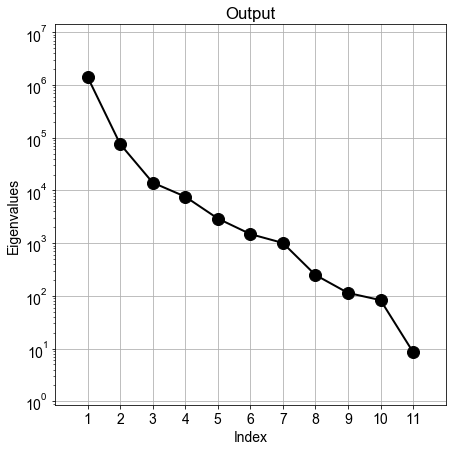
\includegraphics[scale=0.3]{eigs.png} 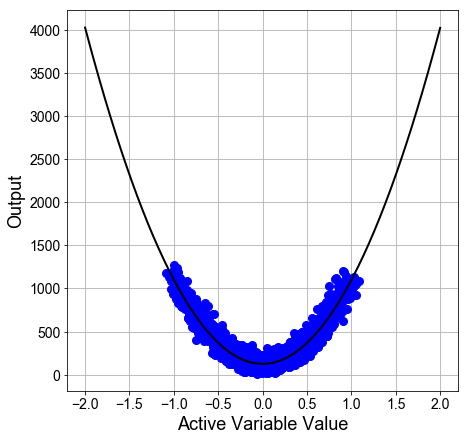
\includegraphics[scale=0.3]{surr.png}

\textbf{Figure 2:} Left: A plot of the eigenvalues of the matrix $\hat{W}$ formed from 1000 Monte Carlo samples in $\Lambda$. We see one dominant eigenvalue on the order of $10^6$. Right: A sufficient summary plot where all 1000 samples are projected into $\A$ and plotted against their function values.
\end{figure} 

We are particularly interested in the quantitative and qualitative difference between active subspaces learned from random sampling versus active subspaces learned from deterministic draws that come from another algorithm such as DFO.


We revisit Example 3, and present two different active subspaces of $f$ -- one active subspace was formed in a Monte Carlo fashion with 1000 random draws in $\Lambda$; the other subspace was formed with only 100 random sample of $f$ where sample points are in fact iterates from a DFO scheme. To consider a realistic scenario, we form the active subspace in both cases by making global quadratic approximations to $\nabla f$, which will work well in our regime since $f$ is quadratic in $\Lambda$.

In Figure 2, we show the results from the first active subspace of $f$, which was obtained from 1000 iid uniform random samples in $[-1,1]^{11}$; i.e., for any sample $\lambda_i$, we have $\lambda_i \sim U[-1,1]^{11}$. The plot on the left-hand side of Figure 2 shows the resulting eigenvalues (the squares of the singular values) from taking the SVD of $\hat{W}$, which we recall is simply a matrix (in this case $1000 \times 10$) where row $i$ is the transpose of approximated gradient of $f$ evaluated at a sample $\lambda_i$, $i=1,\ldots,1000$. Notice that there is one dominating eigenvalue, which is on the order of $10^6$; this matches intuition since the final term in $f(\lambda)$, given by $2^{10}\lambda_{10}^2$, will be, at most, on the order of $10^3$ (and again, eigenvalues are the squares of singular values). This eigenvalue corresponds to $\lambda_{10}$, meaning that the value of $\lambda_{10}$ has the most impact out of all other parameters on the function values $f(\lambda)$. Notice that the eigenvalue near $10^6$ does not dominate the other eigenvalues by much; indeed, another eigenvalue appears around the order $10^5$. Since the second-to-last term in $f$ is small (with coefficient $2^{-9}$), this order $10^5$ eigenvalue must correspond to $2^8\lambda_8^2$.

The active subspace implementation used here \cite{Constantine2015} detects the $10^6$ order eigenvalue as dominating enough to determine that $\A$ is one-dimensional, spanned by the singular vector corresponding to the direction $(0,\ldots,0,1)$, which is a unit vector in the axis of $\lambda_{10}$, orthogonal to all other axes in $\Lambda$.

The plot on the right-hand side of Figure 2 shows the sufficient summary plot, where the 1000 samples are projected into $\A$ using \eqref{eq:7} and their values are plotted along the horizontal axis against their original function values on the vertical axis. The sufficient summary plot can be thought of as a visualization of $f$ along the axes for which $f$ is active; thus, we are seeing a quadratic response in $f$ versus points projected onto the $\lambda_{10}$ axis. We use the mentioned software tools to fit the response with a polynomial surrogate, which is a fit where $R^2\approx 0.9$. Indeed, points do not fall perfectly along the surrogate since there are other parameters which contribute to the value of $f$.

Now we investigate the effectiveness of learning $\A$ with different samples. Since we want to avoid evaluating $f$ heavily and we want to perform several analyses of $f$, it will be advantageous to ``recycle" function values whenever possible. 



To experiment, we consider trying to learn $\A$ from 100 iterates and their function values generated from performing the DFO algorithm STARS \cite{CW} on $f$.  The iterates generated from a DFO algorithm may make large jumps (limited by a step size and smoothing parameter) through regions of $\Lambda$ space early in the routine, but will begin to take smaller and smaller steps as the routine hones in on a local minimum. We note that typically for a fair comparison between sampling methods, one would use the same number of samples; however, we choose to use much less samples in the DFO case for the exact reason that the samples will cease to explore parameter space in an informative manner once the iterates begin to converge to a local minimum. In Figure 3, we present the sufficient plot obtained from learning $\A$ from 100 DFO samples. The eigenvalue plot obtained from the analysis was virtually identical to that in Figure 2, but the sufficient summary plot here in Figure 3 looks very different than the plot in Figure 2 since the sampled points were not random, but deterministic. Notice that the large function value occurs in the top-left corner of the sufficient summary plot in Figure 3; this value corresponds to the initial iterate $\lambda^{(0)}$, which had a function value of approximately 460. Iterates drive down the value of $f$, and we see that the large majority of the iterates (samples) occur in the bottom-right corner of the plot, where the DFO algorithm is converging to a local minimum.


\begin{figure} 
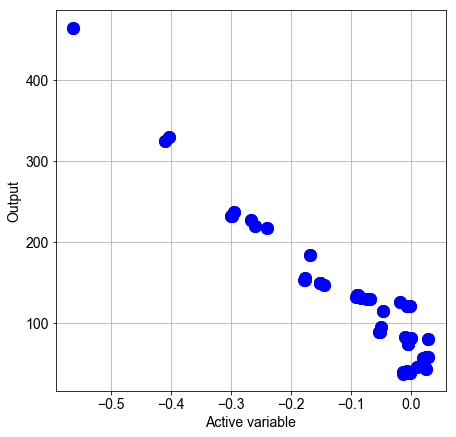
\includegraphics[scale=0.3]{suffsum.png}

\textbf{Figure 3:} A sufficient summary plot where all 100 samples are iterates from a DFO algorithm. 
\end{figure} 

We find that in our case the samples generated from the DFO algorithm explored $\Lambda$ enough to give an active subspace with negligible differences to that obtained in the case of 1000 Monte Carlo draws.

We are interested in exploring the extent to which $\A$ can be learned for more general functions $f$, particularly those arising in certain applications. We are also interested in learning the $L_1$ Lipschitz constant of $f$ in this setting. For the example analyzed here, the step size and smoothing parameters, which are functions of the value of $L_1$, were formed heuristically. A more careful analysis is left to be desired, especially in the case that $\nabla f$ is inaccessible so that $L_1$ must be estimated. Techniques in the literature need to be considered and tested. 



\subsection{Using the Active Subspace} We are generally interested in using the active subspace of a function whenever it may reduce %cheapen
computational expense while maintaining a representations that does not deviate too far from the true action of $f$. Here we consider the effectiveness of DFO performed on $f$ from Example 3 in a standard way \cite{CW} using 500 iterations versus a scheme that blends STARS and active subspace analysis using only 150 iterations. 



We find that after 500 iterations of the standard DFO implementation the routine closes in on the minimum value of $f$, finding that $f\left(\lambda^{(500)}\right) \approx 0.84$. In Figure 4, the left-hand plot shows a \textit{log-log} plot of the logarithm of the iteration on the horizontal axis against the logarithm of the function evaluated at that iterate. We begin to see convergence to a minimum in 500 iterations.
We modified the DFO algorithm to find a similar result with only 150 iterations. 

To make a modified DFO routine, we begin with a ``burn in" of 50 iterations of standard DFO, which actually gives 100 samples of the function at different points in $\Lambda$, as one step of the DFO routine has two calls of $f$. From the 100 samples denoted with $D$, we form $\A(f,D)$. The results of this analysis were discussed above; recall, we obtain a one-dimensional $\A$ spanned in the direction of $\lambda_{10}$. Though $\A$ is one-dimensional, there are still other important parameters in the model, including $\lambda_8$ and $\lambda_6$, which make order $10^2$ and $10^1$ contributions to $f$ respectively. After the standard DFO burn-in, which was used to both minimize $f$ and explore $\Lambda$ to obtain an approximate $\A$, we begin to use DFO only in the directions of the active and some inactive variables. Since we have only a single direction to minimize along in the active subspace, we modify the DFO algorithm to take random steps in the direction of the $\lambda_{10}$ axis only. We do so by taking draws from a $ d \sim N(0,1)$ and forming the randomly scaled vector $du_1$, where $u_1$ is the singular vector corresponding to the active direction in $\lambda_{10}$. Now, each iterate will only be perturbed in its last component in the DFO scheme. We find that in this example, the STARS burn-in phase reduces the 10th component of iterates so that $\lambda^{(50)}_{10} \approx -0.01$ and $f(\lambda^{(50)})\approx 38.02$. Performing DFO in the $\lambda_{10}$ axis with 25 iterations gives $\lambda^{(75)}_{10}$ on the order of $10^{-4}$, but $f(\lambda^{(75)}) \approx 37.74$, which is only a small drop in the function value. Next, 25 iterations of DFO was performed along the $\lambda_8$ axis -- this time, we see a significant drop in the value of $f$, where $f^{(100)} \approx 29.34$. Despite the fact that the $\lambda_8$ direction is not considered active, we do see the value of $f$ decrease as $f$ is minimized along its axis. Another 25 iterations of DFO was performed along the direction corresponding to the third singular vector, dropping the value of $f$ by about 6. Finally, 25 iterations of DFO was performed along the axis corresponding to the fourth singular vector, which minimizes $f$ to an order similar to the results from 500 iterations of standard DFO. Indeed, $f(\lambda^{(150)})\approx 1.38$.

\begin{figure} 
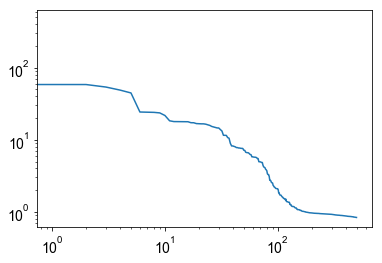
\includegraphics[scale=0.3]{stars.png} 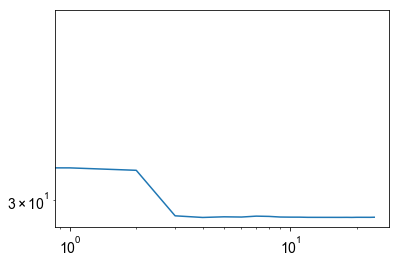
\includegraphics[scale=0.3]{minvec2.png} 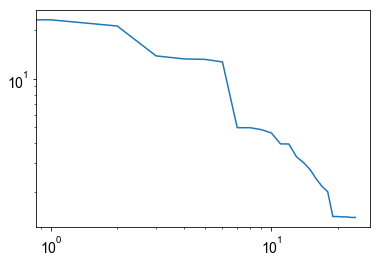
\includegraphics[scale=0.3]{minvec4.png}

\textbf{Figure 4:} 3 log-log plots from (left to right): 500 iterations of standard DFO; 25 iterations of minimizing $f$ with DFO along the $\lambda_8$ axis; 25 iterations of minimizing $f$ with DFO along the $\lambda_6$ axis.
\end{figure} 

In the middle plot of Figure 4, we show the log-log plot obtained from using 25 steps of DFO in the $\lambda_8$ direction; the right-hand log-log plot shows the results of 25 steps of DFO in the $\lambda_6$ direction.


We note that we have presented just one of several algorithms that have in some way blended the active subspace of $f$ with a DFO scheme. We are interested in investigating the best way to use the information of $\A$ in DFO. Likewise, we are interested in representing $f$ with surrogates based on $\A$ and investigating whether $\A$ can lessen the computational expense in the forward problem.

\subsection{From model problems to fusion applications}

We propose to investigate the approximate solution of data-consistent inverse problems via optimization approaches.  For derivative free optimization, we plan to transition from our noisy
functions to the data consistent inversion of a subgrid LES model for isotropic turbulent flow.  
While this would certainly be a publishable result, the hope is to investigate approximate DCI
when applied to anomalous diffusion in the axisymmetric gyrokinetic code XGCa.

In the case of models where $\lambda$-gradients are available and not of suspect quality, we will
transition from an approximate DCI for a model elliptic problem with a parameterized forcing function, with parameter gradients obtained via adjoint methods.  Success here will allow us to extend the
method to the determination of data-consistent MHD equilibria (via the Grad-Shafranov equation).  





\subsection{Software Dissemination}

Currently, only some of the software used to produce results in this paper are publicly available on GitHub.com. Some of the algorithms used here and other algorithms that are of interest are within open-source packages available online including those of Constantine and Butler et al. Other schemes considered in this paper make modifications to given algorithms and remain under development. A major goal of this thesis proposal will be developing well-documented, open-source software complete with python Jupyter Notebooks and illustrative, replicable examples.

\section{Timeline}

We outline a rough timeline for the remaining 2 years in a 5.5 year plan.

\begin{itemize}

\item Clean existing algorithms and examples, generate richer research results related to DFO and active subspaces, and build a model inverse problem for investigation. (Dec 2018/Jan 2019)

\item On RA for Spring 2019.

\item Write and present MS-level results. (Feb/Mar 2019)

\item Work on theoretical formulation of deregularization for nonlinear $f$. Work on generating notebooks and examples. (Ongoing/Spring and Summer 2019)

\item Summer research; begin writing thesis; summer school/internship/conference. (Jun/Jul/Aug 2019)

\item Fall 2019 - Writing phase, revisions.

\item Spring 2020 - Final revisions, software.

\item Summer 2020 Internship/collaborations, publishing, formatting.

\item Defend thesis Summer 2020 or early Fall 2020.


\end{itemize}


%%%%%%%%%%%%%% References %%%%%%%%%%%%%%%%%%%%%%%%%
\begin{thebibliography}{65}

\bibitem{battaglia} Battaglia, D. J.  and Burrell, K. H.  and Chang, C. S.  and Ku, S.  and deGrassie, J. S.  and Grierson, B. A. ``Kinetic neoclassical transport in the H-mode pedestal." Physics of Plasmas,Volume 21, No. 7. 2014.


\bibitem{BJW18a} T. Butler and J. Jakeman and T. Wildey.
``Combining Push-Forward Measures and Bayes' Rule to Construct Consistent Solutions to Stochastic Inverse Problems." SIAM Journal on Scientific Computing, Volume 40, No. 2, pp. A984-A1011, 2018.

\bibitem{Calliess} Jan-Peter Calliess. ``Lipschitz optimisation for Lipschitz interpolation." In 2017 American Control Conference (ACC 2017), Seattle, WA, USA, May 2017.

\bibitem{CW} Chen and Wild. ``Randomized Derivative-Free Optimization of Noisy Convex Functions." Funded by the Department of Energy. 2015.

\bibitem{Constantine2015} Constantine, Paul G. ``Active Subspaces: Emerging Ideas for Dimension Reduction in Parameter Studies." SIAM, 2015.

\bibitem{ConstantineMC} Constantine, Eftekhari, Wakin. ``Computing Active Subspaces Efficiently with Gradient Sketching." Conference paper, 2015 IEEE 6th International Workshop on Computational Advances in Multi-Sensor Adaptive Processing (CAMSAP).


\bibitem{KS} Kvasov and Sergeyev. ``Lipschitz gradients for global optimization in a one-point-based partitioning scheme." Journal of Computational and Applied Mathematics. Volume 236, Issue 16, pp. 4042-4054. 2012.

\bibitem{KU_TOTALF} S. Ku and R. Hager and C.S. Chang and J.M. Kwon and S.E. Parker. ``A new hybrid-Lagrangian numerical scheme for gyrokinetic simulation of tokamak edge plasma." Journal of Computational Physics, Volume 315, pp. 467-475. 2016.

\bibitem{Lao85} Lao, L.L, St. John, H, R.D. Stambaugh, A.G. Kellman, and Pfeiffer, W.,``Reconstruction of current profile parameters and plasma shapes in tokamaks'', Nuclear Fusion, Volume 25,No. 11,pp. 1611,1985.

\bibitem{lea2000} Lea, Daniel J. and Allen, Myles R. and Haine, Thomas W. N. ``Sensitivity analysis of the climate of a chaotic system." Tellus A, Volume 52, No. 5, pp. 523-532. 2000.






\bibitem{Russi} Russi, Trent M. ``Uncertainty Quantification with Experimental Data and Complex System Models." Dissertation, University of California Berkeley. 2010.

\bibitem{Smith}  Smith, Ralph.``Uncertainty Quantification: Theory, Implementation, and Applications.” SIAM, 2013.

\bibitem{Stuart} Stuart, Andrew. ``Inverse problems: A Bayesian perspective." Acta Numerica, volume 19, pp. 451-559. 2010.



\bibitem{Tarantola} Tarantola, Albert. ``Inverse Problem Theory and Methods for Model Parameter Estimation." SIAM. 2005.

\bibitem{Takeda91} Takeda, T. and Tokuda S.,``Computation of MHD equilibrium of tokamak plasma'',
Journal of Computational Physics,93,1,1 - 107,1991.

\bibitem{Qiqi2014} Qiqi Wang and Rui Hu and Patrick Blonigan. ``Least Squares Shadowing sensitivity analysis of chaotic limit cycle oscillations." Journal of Computational Physics, Volume 267, pp. 210-224. 2014.


\bibitem{Wesson} Wesson, J. ``Tokamaks." ``Oxford University Press, 4th edition." 2011.

\bibitem{wildeyprez} Wildey, T., Butler, T., Jakeman, J., Walsh, S. " A Consistent Bayesian Approach for Stochastic Inverse Problems Based on Push-forward Measures." SAND2017-3436PE. 2017.


\end{thebibliography}




\end{document}
